%% ============================================================
%%  CORRECTED main.tex  — preamble and CHAPTER I only
%%  For the rest of the document (chapters II-VI, back matter)
%%  keep your existing content unchanged.
%% ============================================================

\documentclass[a4paper,12pt,oneside]{book}

%% --- Font: times is declared in package-settings.tex ---
%% REMOVED: \usepackage{tgtermes}  (duplicate font — conflicts)
%% REMOVED: \usepackage[cmex10]{amsmath} (duplicate — in package-settings)
%% REMOVED: \usepackage{amssymb}   (duplicate — in package-settings)
%% REMOVED: \usepackage{mathabx}   (conflicts with amssymb — causes
%%          "already defined" errors in Overleaf and pdflatex)

\usepackage{booktabs}
\usepackage{multirow}
\usepackage{graphicx}
\graphicspath{{Figures/}}
\usepackage{array}
\usepackage{algorithm}
\usepackage{float}
\usepackage{tabularx}
\usepackage{setspace}
\usepackage{tikz}
%% NOTE: TikZ libraries only needed if you use TikZ drawings.
%% If you draw diagrams externally (as images), you may remove
%% the next line safely.
\usetikzlibrary{arrows.meta,positioning,shapes.geometric,calc,backgrounds}
\usepackage{xcolor}
\usepackage{pdfpages}
\usepackage{rotating}
\usepackage{colortbl}
\usepackage{url}

%% Define custom hyperlink colours
\definecolor{mylinkcolor}{RGB}{0,0,0}
\definecolor{toclinkcolor}{RGB}{0,0,0}

% ====================== package-settings.tex (CLEANED) ======================
\usepackage[T1]{fontenc}
\usepackage[utf8]{inputenc}
\usepackage{times} 
\usepackage{amsfonts,amsmath,amsthm,amssymb}
\usepackage{graphicx}
\usepackage{caption}
\usepackage{booktabs}
\usepackage{longtable}
\usepackage{threeparttable}
\usepackage{subcaption}
\usepackage{algorithmic}
\usepackage{textcomp}
\usepackage{multicol}
\usepackage{multirow}
\usepackage{adjustbox}
\usepackage{appendix}
\usepackage{enumitem}
\usepackage{array}
\usepackage{calc}
\usepackage{setspace}
\usepackage{tocloft}
\usepackage[explicit]{titlesec}
\usepackage{parskip}
\setlength{\emergencystretch}{2em}

% ====================== IEEE BIBLIOGRAPHY (biblatex) ======================
\usepackage[
  backend=biber,
  style=ieee,
  sorting=none,
  giveninits=true
]{biblatex}
\addbibresource{references.bib}

% ====================== HYPERREF (must be last) ======================
\usepackage[hidelinks]{hyperref}
\usepackage{bookmark}
\hypersetup{colorlinks=true, linkcolor=black, citecolor=black, urlcolor=black}

% ====================== KUET CHAPTER/SECTION STYLE ======================
\renewcommand{\thechapter}{\Roman{chapter}}
\renewcommand{\thesection}{\arabic{chapter}.\arabic{section}}
\renewcommand{\theequation}{\arabic{chapter}.\arabic{equation}}
\renewcommand{\thefigure}{\arabic{chapter}.\arabic{figure}}
\titleformat{\chapter}[display]{\normalfont\large\bfseries\filcenter}{\MakeUppercase\chaptertitlename\ \thechapter}{40pt}{{#1}}
\titlespacing*{\chapter}{0pt}{-30pt}{40pt}
\titleformat{\section}{\normalfont\large\bfseries}{\thesection}{0.65em}{#1}
\titlespacing*{\section}{0pt}{3.5ex plus 1ex minus .2ex}{1ex plus .2ex}
\titleformat{\subsection}{\normalfont\normalsize\bfseries}{\thesubsection}{0.65em}{#1}
\titlespacing*{\subsection}{0pt}{3.25ex plus 1ex minus .2ex}{0.8ex plus .2ex}

% ====================== LINE SPACING ======================
\usepackage{setspace}
\setstretch{1.5}

% ====================== TOC / LOF / LOT ======================
\renewcommand{\cfttoctitlefont}{\hfill\large\bfseries}
\renewcommand{\cftaftertoctitle}{\hfill}
\addtocontents{toc}{~\hfill\textbf{Page}\par}
\setlength{\cftbeforepartskip}{2pt}
\setlength{\cftbeforechapskip}{8pt}
\setlength{\cftbeforesecskip}{1pt}
\setlength{\cftbeforesubsecskip}{0pt}
\setlength{\cftpartindent}{2.8em}
\setlength{\cftchapindent}{0pt}
\setlength{\cftsecindent}{8.5em}
\setlength{\cftsubsecindent}{11.3em}
\setlength{\cftpartnumwidth}{0pt}
\setlength{\cftchapnumwidth}{8.5em}
\setlength{\cftsecnumwidth}{3em}
\setlength{\cftsubsecnumwidth}{4em}
\renewcommand{\cftpartfont}{\normalfont}
\renewcommand{\cftpartpagefont}{\normalfont}
\renewcommand{\cftchapfont}{\normalfont}
\renewcommand{\cftchappagefont}{\normalfont}
\renewcommand{\cftsecfont}{\normalfont}
\renewcommand{\cftsecpagefont}{\normalfont}
\renewcommand{\cftsubsecfont}{\normalfont}
\renewcommand{\cftsubsecpagefont}{\normalfont}
\renewcommand{\cftchappresnum}{\bfseries CHAPTER\ }
\renewcommand{\cftchapaftersnum}{\normalfont\quad}
\renewcommand{\cftchapleader}{\hfill}
\renewcommand{\cftpartleader}{\hfill}
\renewcommand{\cftsecleader}{\hfill}
\renewcommand{\cftsubsecleader}{\hfill}
\renewcommand{\cftlottitlefont}{\hfill\large\bfseries\MakeUppercase}
\renewcommand{\cftafterlottitle}{\hfill}
\renewcommand{\cftloftitlefont}{\hfill\large\bfseries\MakeUppercase}
\renewcommand{\cftafterloftitle}{\hfill}
\renewcommand{\cftsecdotsep}{\cftnodots}
\renewcommand{\cftsubsecdotsep}{\cftnodots}
\renewcommand{\cftfigdotsep}{\cftnodots}
\renewcommand{\cfttabdotsep}{\cftnodots}


%% Override hyperref colour (must come AFTER % ====================== package-settings.tex (CLEANED) ======================
\usepackage[T1]{fontenc}
\usepackage[utf8]{inputenc}
\usepackage{times} 
\usepackage{amsfonts,amsmath,amsthm,amssymb}
\usepackage{graphicx}
\usepackage{caption}
\usepackage{booktabs}
\usepackage{longtable}
\usepackage{threeparttable}
\usepackage{subcaption}
\usepackage{algorithmic}
\usepackage{textcomp}
\usepackage{multicol}
\usepackage{multirow}
\usepackage{adjustbox}
\usepackage{appendix}
\usepackage{enumitem}
\usepackage{array}
\usepackage{calc}
\usepackage{setspace}
\usepackage{tocloft}
\usepackage[explicit]{titlesec}
\usepackage{parskip}
\setlength{\emergencystretch}{2em}

% ====================== IEEE BIBLIOGRAPHY (biblatex) ======================
\usepackage[
  backend=biber,
  style=ieee,
  sorting=none,
  giveninits=true
]{biblatex}
\addbibresource{references.bib}

% ====================== HYPERREF (must be last) ======================
\usepackage[hidelinks]{hyperref}
\usepackage{bookmark}
\hypersetup{colorlinks=true, linkcolor=black, citecolor=black, urlcolor=black}

% ====================== KUET CHAPTER/SECTION STYLE ======================
\renewcommand{\thechapter}{\Roman{chapter}}
\renewcommand{\thesection}{\arabic{chapter}.\arabic{section}}
\renewcommand{\theequation}{\arabic{chapter}.\arabic{equation}}
\renewcommand{\thefigure}{\arabic{chapter}.\arabic{figure}}
\titleformat{\chapter}[display]{\normalfont\large\bfseries\filcenter}{\MakeUppercase\chaptertitlename\ \thechapter}{40pt}{{#1}}
\titlespacing*{\chapter}{0pt}{-30pt}{40pt}
\titleformat{\section}{\normalfont\large\bfseries}{\thesection}{0.65em}{#1}
\titlespacing*{\section}{0pt}{3.5ex plus 1ex minus .2ex}{1ex plus .2ex}
\titleformat{\subsection}{\normalfont\normalsize\bfseries}{\thesubsection}{0.65em}{#1}
\titlespacing*{\subsection}{0pt}{3.25ex plus 1ex minus .2ex}{0.8ex plus .2ex}

% ====================== LINE SPACING ======================
\usepackage{setspace}
\setstretch{1.5}

% ====================== TOC / LOF / LOT ======================
\renewcommand{\cfttoctitlefont}{\hfill\large\bfseries}
\renewcommand{\cftaftertoctitle}{\hfill}
\addtocontents{toc}{~\hfill\textbf{Page}\par}
\setlength{\cftbeforepartskip}{2pt}
\setlength{\cftbeforechapskip}{8pt}
\setlength{\cftbeforesecskip}{1pt}
\setlength{\cftbeforesubsecskip}{0pt}
\setlength{\cftpartindent}{2.8em}
\setlength{\cftchapindent}{0pt}
\setlength{\cftsecindent}{8.5em}
\setlength{\cftsubsecindent}{11.3em}
\setlength{\cftpartnumwidth}{0pt}
\setlength{\cftchapnumwidth}{8.5em}
\setlength{\cftsecnumwidth}{3em}
\setlength{\cftsubsecnumwidth}{4em}
\renewcommand{\cftpartfont}{\normalfont}
\renewcommand{\cftpartpagefont}{\normalfont}
\renewcommand{\cftchapfont}{\normalfont}
\renewcommand{\cftchappagefont}{\normalfont}
\renewcommand{\cftsecfont}{\normalfont}
\renewcommand{\cftsecpagefont}{\normalfont}
\renewcommand{\cftsubsecfont}{\normalfont}
\renewcommand{\cftsubsecpagefont}{\normalfont}
\renewcommand{\cftchappresnum}{\bfseries CHAPTER\ }
\renewcommand{\cftchapaftersnum}{\normalfont\quad}
\renewcommand{\cftchapleader}{\hfill}
\renewcommand{\cftpartleader}{\hfill}
\renewcommand{\cftsecleader}{\hfill}
\renewcommand{\cftsubsecleader}{\hfill}
\renewcommand{\cftlottitlefont}{\hfill\large\bfseries\MakeUppercase}
\renewcommand{\cftafterlottitle}{\hfill}
\renewcommand{\cftloftitlefont}{\hfill\large\bfseries\MakeUppercase}
\renewcommand{\cftafterloftitle}{\hfill}
\renewcommand{\cftsecdotsep}{\cftnodots}
\renewcommand{\cftsubsecdotsep}{\cftnodots}
\renewcommand{\cftfigdotsep}{\cftnodots}
\renewcommand{\cfttabdotsep}{\cftnodots}
)
\hypersetup{
  colorlinks=true,
  linkcolor=mylinkcolor,
  citecolor=mylinkcolor,
  urlcolor=mylinkcolor,
}

%%%% Custom commands %%%%
\newcommand{\blanklineR}{\hfill \\}
\newcommand{\HeadingR}[1]{{\large\bfseries{#1}}}
\newcommand{\titleR}{System Identification and PID Control of a Line-Following Robot}
\newcommand{\safeincludegraphics}[3][]{%
  \IfFileExists{#2}{%
    \includegraphics[#1]{#2}%
  }{%
    \fbox{%
      \parbox[c][0.22\textheight][c]{0.85\textwidth}{%
        \centering\textbf{Figure placeholder}\\[0.5ex]
        Missing file: \texttt{\detokenize{#2}}\\[0.5ex]
        #3%
      }%
    }%
  }%
}

%%%% PDF metadata %%%%
\hypersetup{%
  pdfauthor={SIMUL AHMED},
  pdftitle=\titleR,
  pdfsubject={B.Sc. Eng. Project},
  pdfkeywords={}
}

%%%%%%%%%%%%%%%%%%%%%%%%%%%%%%%%%%%%%%%%%%%%%%%%%%%%%%%%%%%%
%%  DOCUMENT
%%%%%%%%%%%%%%%%%%%%%%%%%%%%%%%%%%%%%%%%%%%%%%%%%%%%%%%%%%%%
\begin{document}
\frontmatter

%% --- Title Page ---
\hypersetup{pageanchor=false}
\begin{titlepage}
\phantomsection
\addcontentsline{toc}{part}{Title Page}
\centering
\HeadingR{\MakeUppercase{\titleR}}
\blanklineR\blanklineR\blanklineR
{\fontsize{16}{12}\selectfont \textbf{Submitted By:}}\\
\blanklineR
{\fontsize{14}{12}\selectfont \MakeUppercase{SIMUL AHMED} \hspace{1.15cm} \MakeUppercase{ROLL NO. 2113006}}
\blanklineR\blanklineR\blanklineR
{\fontsize{16}{12}\selectfont \textbf{Submitted To:}}\\
\blanklineR
{\fontsize{14}{12}\selectfont \MakeUppercase{Mostafizur Rahaman}\\
\MakeUppercase{Lecturer}}\\
\blanklineR\blanklineR\blanklineR

\includegraphics[width=0.26\textwidth]{Figures/kuet_logo.jpg}
\blanklineR\blanklineR
{\fontsize{14}{12}\selectfont A Project report submitted to the Department of Energy Science and Engineering, Khulna University of Engineering \& Technology, Khulna in partial fulfillment of the requirements for the degree of \textbf{\textit{``Bachelor of Science in Energy Science and Engineering''}}}
% \blanklineR\blanklineR\blanklineR
\textbf{April 2026}
\end{titlepage}
\hypersetup{pageanchor=true}

%% --- Abstract ---
\newpage
\phantomsection \label{abstr}
\addcontentsline{toc}{part}{Abstract}
\begin{center}
\HeadingR{\MakeUppercase{Abstract}}
\end{center}


This project presents the system identification and PID control of a differential-drive line-following robot. The robot was developed using an Arduino Nano, a 14-element infrared sensor array, an L298N motor driver, and two DC motors. A weighted centre-of-mass method was used to estimate line position, and the resulting tracking error was used as the feedback signal.

Experimental data were collected from the physical robot through Bluetooth telemetry. The plant input was defined as the differential steering command, and the plant output was taken as the measured tracking error. From these data, a second-order discrete-time transfer-function model with a sampling time of 0.05~s was identified.

The identified model was implemented in MATLAB/Simulink for PID tuning. The tuned controller was then deployed to the robot and tested on the track. Simulation showed stable closed-loop behaviour, while hardware tests confirmed successful line following. Although the real response was affected by motor dead-zone, saturation, and sensor quantisation, the study shows that transfer-function identification and simulation-based PID tuning provide a systematic alternative to manual controller tuning for a low-cost line-following robot.


\textbf{Keywords:} line-following robot, PID control, system identification, differential-drive, transfer function

%% --- Table of Contents ---
\newpage
\renewcommand\contentsname{CONTENTS}
\addcontentsline{toc}{part}{Contents}
\begin{singlespacing}
{\hypersetup{linkcolor=black}
\tableofcontents
}
\end{singlespacing}

%% --- List of Tables ---
% \newpage
% \phantomsection \label{listoftab}
% \addcontentsline{toc}{part}{List of Tables}
% {\hypersetup{linkcolor=black}
% \listoftables
% }
% \addtocontents{lot}{\textbf{Table No}\hfill \textbf{Description}\hfill\textbf{Page}\par}

%% --- List of Figures ---
\newpage
\phantomsection \label{listoffig}
\addcontentsline{toc}{part}{List of Figures}
{\hypersetup{linkcolor=black}
\listoffigures
}
\addtocontents{lof}{\textbf{Figure No}\hfill \textbf{Description}\hfill\textbf{Page}\par}

\mainmatter
\bookmarksetup{startatroot}
\newpage
%% ============================================================
%%  CHAPTER I — INTRODUCTION
%% ============================================================

\chapter{INTRODUCTION}\label{chap:intro}

\section{General}

Line-following robots are widely used as low-cost platforms for studying sensing,
path tracking, and feedback control in structured environments
\cite{balaji2015}. A common configuration is the differential-drive robot, in
which steering is produced by creating a speed difference between the left and
right wheels \cite{siwek2023}. In such systems, the main control objective is to
reduce the lateral position error of the robot relative to the line. This error
can be estimated in real time from an infrared sensor array mounted at the front
of the robot \cite{baharuddin2006}.

Because the robot does not naturally return to the line after a disturbance,
proportional action alone is often not sufficient for satisfactory tracking.
Therefore, PID control is a practical choice for improving line-following
performance \cite{balaji2015}.

\subsection{The PID Controller}

PID control is widely used because of its simple structure and practical
effectiveness in embedded systems \cite{borase2020}. In the present work, the
controller acts on the measured tracking error and generates a steering command
for the differential-drive robot. The continuous-time PID law is

\begin{equation}
    u(t) \;=\; K_P\,e(t)
             \;+\; K_I\!\int_{0}^{t}\!e(\tau)\,\mathrm{d}\tau
             \;+\; K_D\,\frac{\mathrm{d}e(t)}{\mathrm{d}t}
    \label{eq:pid}
\end{equation}

\noindent
where \(e(t)=r-y(t)\) is the control error and \(K_P\), \(K_I\), and \(K_D\) are
the proportional, integral, and derivative gains, respectively.
Figure~\ref{fig:pid_structure} shows the parallel form of the PID controller.

\begin{figure}[htbp]
    \centering
    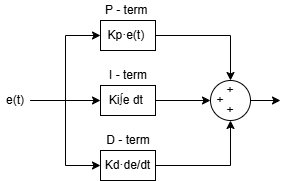
\includegraphics[width=0.72\textwidth]{Figures/fig_pid_structure.png}
    \caption[Internal parallel structure of the PID controller.]%
    {Internal parallel structure of the PID controller.}
    \label{fig:pid_structure}
\end{figure}

A standard feedback arrangement is shown in Figure~\ref{fig:pid_closedloop}.
For line-following applications, proportional action gives the basic steering
response, while integral and derivative actions can improve overall tracking
behaviour \cite{balaji2015}.

\begin{figure}[htbp]
    \centering
    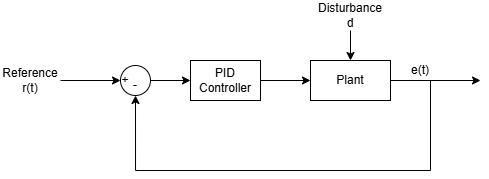
\includegraphics[width=0.85\textwidth]{Figures/fig_pid_closedloop.png}
    \caption[Canonical closed-loop PID control system for DC motor speed regulation.]%
    {Canonical example of a closed-loop PID control system.}
    \label{fig:pid_closedloop}
\end{figure}

For embedded implementation, the controller is discretized at the sampling period
\(T_s\).

\subsection{System Identification and PID Tuning}

Manual tuning is common in small line-following robots, but it does not provide a
systematic description of the robot dynamics \cite{balaji2015,brigido2025}. A
more structured approach is to first identify a mathematical plant model from
measured input-output data and then use that model for controller design
\cite{ljung1999,ljung2010}.

In this project, system identification is used to represent the dynamic relation
between the differential steering command and the measured tracking error. The
robot is tested experimentally, and the recorded data are used to identify a
discrete-time transfer-function model. Figure~\ref{fig:sysid_workflow}
illustrates the general identification concept.

\begin{figure}[htbp]
    \centering
    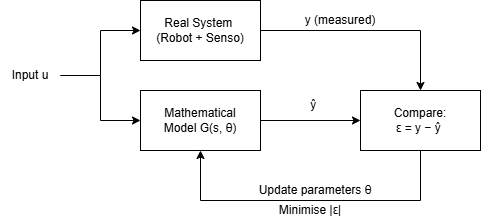
\includegraphics[width=0.82\textwidth]{Figures/fig_sysid_workflow.png}
    \caption[Data-driven system identification workflow.]%
    {Data-driven system identification workflow. The same input \(u\) is applied to
    the real plant and to the candidate model \(\hat{G}(\theta)\), and the model
    parameters are updated to reduce the prediction error between measured and
    estimated output.}
    \label{fig:sysid_workflow}
\end{figure}

Once the plant model is obtained, PID gains can be tuned in simulation before
hardware implementation. In the present work, the identified plant is imported
into MATLAB PID Tuner, and the tuned gains are then deployed to the robot for
experimental testing. This overall procedure is shown in
Figure~\ref{fig:pid_tuning_workflow}.

\begin{figure}[htbp]
    \centering
    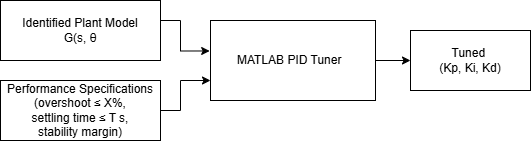
\includegraphics[width=0.82\textwidth]{Figures/fig_pid_tuning_.png}
    \caption[Simulation-based PID tuning workflow.]%
    {Simulation-based PID tuning workflow. The identified plant model is used in
    MATLAB PID Tuner to obtain controller gains before deployment to the physical
    robot.}
    \label{fig:pid_tuning_workflow}
\end{figure}

\section{Specific Objectives}

The specific objectives of this project are as follows:

\begin{enumerate}[label=\roman*., leftmargin=*]

    \item To design, construct, and calibrate a differential-drive line-following
    robot with a 14-element infrared sensor array and to generate a normalised
    tracking error signal for feedback control.

    \item To identify a discrete-time transfer-function model of the robot from
    the collected experimental data.

    \item To tune PID controller gains in MATLAB using the identified model and
    to implement the tuned controller on the Arduino Nano.

    \item To evaluate the closed-loop performance of the tuned controller on the
    physical robot through experimental testing.

\end{enumerate}

%% ============================================================
%%  CHAPTER II onwards — paste your existing chapters below
%% ============================================================

% ================================================================

\newpage
\chapter{LITERATURE REVIEW}
\label{chap:lit_review}

\section{Line-Following Robots and Sensing}

Line-following robots are widely used as simple platforms for studying sensing,
path tracking, and feedback control in structured environments
\cite{brigido2025,balaji2015}.

Reliable line-position estimation is essential for closed-loop tracking.
Baharuddin et al. showed that sensor arrays provide better line detection than a
small number of discrete sensors \cite{baharuddin2006}. Balaji et al. also used
an analogue infrared sensor array to generate a single position-related error
signal suitable for feedback control \cite{balaji2015}. These findings support
the use of a multi-element infrared sensor array and a single lateral error
signal in the present work.

\section{Differential-Drive Modeling and PID Control}

Differential-drive robots are common in line-following applications because
steering can be produced by creating a speed difference between the left and
right wheels \cite{balaji2015}. Siwek et al. highlighted the importance of
dynamic modeling and parameter identification for differential-drive robots when
plant behaviour cannot be described accurately from physical specifications
alone \cite{siwek2023}. This supports the use of experimentally identified
models for controller design.

PID control remains a practical choice for embedded robotic systems because of
its simple structure, low computational cost, and wide engineering use
\cite{borase2020}. In line-following robots, Balaji et al. showed that
trial-and-error control becomes less effective as the system becomes faster and
more demanding, while PID control offers a more systematic approach
\cite{balaji2015}.

\section{PID Tuning and System Identification}

Classical PID tuning methods such as Ziegler--Nichols and related auto-tuning
approaches remain important in control engineering
\cite{ziegler1942,astrom1984,hang2002}. However, these general methods do not
always reflect the actual behaviour of a small mobile robot operating with
sensor-based feedback and actuator limits. In many practical line-following
systems, gains are still chosen manually \cite{balaji2015}.

System identification provides a systematic way to build a mathematical model
from measured input-output data \cite{ljung1999,ljung2010}. This is useful when
the plant dynamics are difficult to obtain directly from theoretical analysis.
In the present work, this idea is applied by identifying a discrete-time
transfer function from real robot data and then using that model for
simulation-based PID tuning in MATLAB.

\section{Research Gap and Motivation}

The literature shows that line-following robots are widely studied and that PID
control is a practical solution for embedded implementation. However, many
low-cost systems still rely mainly on heuristic tuning instead of combining
experimental plant identification with controller design
\cite{balaji2015,brigido2025}.

The present work is motivated by the need for a more systematic workflow for a
low-cost line-following robot, combining sensor calibration, experimental data
collection, transfer-function identification, simulation-based PID tuning, and
hardware validation on the real robot.

% ================================================================

% ================================================================
\newpage
\chapter{METHODOLOGY}\label{chap:methodology}

\section{Hardware Architecture and System Overview}

The experimental platform used in this study was a custom-built differential-drive
line-following robot developed for sensor-based tracking and embedded control.
The main hardware components were an Arduino Nano microcontroller, an L298N
dual H-bridge motor driver, a 14-element infrared reflectance sensor array, a
Bluetooth serial module for telemetry, two N20 geared DC motors, and a Li-Po
battery supply. Figure~\ref{fig:hardware_block} shows the overall hardware
architecture of the system.

\begin{figure}[htbp]
    \centering
    \safeincludegraphics[width=0.9\textwidth]{Figures/Diagram LFR-Page-7.drawio.png}{Complete hardware block diagram.}
    \caption{Complete hardware block diagram showing the power supply, Arduino
    Nano, multiplexer-assisted sensor interface, L298N motor driver, DC motors,
    and Bluetooth telemetry link.}
    \label{fig:hardware_block}
\end{figure}

The Arduino Nano acted as the central controller. During each control cycle, it
read the sensor array, estimated the line position error, computed the control
signal, and updated the motor commands. Because the 14 analogue sensor outputs
were read sequentially through a multiplexer and telemetry was transmitted
through Bluetooth, the loop interval was not perfectly constant. In practice, the
average sampling interval was approximately \(50~\mathrm{ms}\).

The line sensor array was mounted at the front of the robot and arranged
symmetrically about the centreline. The sensor positions were labelled from
\(-7\) to \(-1\) on the left side and from \(+1\) to \(+7\) on the right side,
with no physical sensor at the exact centre. The sensor layout is shown in
Figure~\ref{fig:sensor_layout}.

\begin{figure}[htbp]
    \centering
    \safeincludegraphics[width=0.85\textwidth]{Figures/bot_diagram.png}{Top-view layout of the sensor array.}
    \caption{Top-view layout of the 14-element infrared sensor array with position
    labels from \(-7\) (far left) to \(+7\) (far right), excluding the physical
    centre position.}
    \label{fig:sensor_layout}
\end{figure}

The wheel motors were driven through the L298N H-bridge. Motor commands were
expressed in the range \([-100,+100]\), where positive values represented
forward motion and negative values represented reverse motion. In practice, the
motors showed a dead-zone around zero command because of friction and driver
limitations. Reliable motion was not observed for very small command values,
approximately within \([-15,+15]\).

A Bluetooth serial module was used to transmit telemetry from the robot to a host
computer. The transmitted data included time stamp, left motor command, right
motor command, and measured tracking error. The assembled robot used in the
experimental study is shown in Figure~\ref{fig:robot_photo}.

\begin{figure}[htbp]
    \centering
    \safeincludegraphics[width=0.75\textwidth]{Figures/IMG_20260404_193412186_AE.jpg.jpeg}{Photograph of the assembled robot.}
    \caption{Photograph of the assembled differential-drive line-following robot
    used in the experimental study.}
    \label{fig:robot_photo}
\end{figure}

\section{Sensor Calibration and Error Estimation}

Before each experimental run, all 14 infrared sensors were calibrated using
uniform white and black reference surfaces. For each sensor \(i\), the average
white reading \(\mu_{w,i}\) and average black reading \(\mu_{b,i}\) were
measured, and the decision threshold was defined as

\begin{equation}
    T_i=\frac{\mu_{w,i}+\mu_{b,i}}{2}.
    \label{eq:sensor_threshold}
\end{equation}

This threshold compensated for sensor-to-sensor variation in gain and offset.
The calibration result is shown in Figure~\ref{fig:sensor_cal}.

\begin{figure}[htbp]
    \centering
    \safeincludegraphics[width=0.9\textwidth]{Figures/sersor cal.png}{Sensor calibration results.}
    \caption{Calibration results of the 14-element infrared sensor array, showing the average white reading, average black reading, and threshold for each sensor position. The annotated \(D_i\) values indicate the contrast between the two surfaces.}
    \label{fig:sensor_cal}
\end{figure}

At each control cycle, the raw reading of each sensor was compared with its
threshold to produce a binary detection signal \(w_i \in \{0,1\}\). The lateral
line position was then estimated by a weighted centre-of-mass calculation,

\begin{equation}
    e_{\mathrm{raw}}=
    \frac{\sum_{i=1}^{14} p_i\,w_i}
         {\sum_{i=1}^{14} w_i},
    \label{eq:raw_error}
\end{equation}

\noindent
where \(p_i\) is the position assigned to sensor \(i\). The sensor positions were
defined as \(\{-7,-6,\ldots,-1,+1,\ldots,+7\}\), consistent with the physical
layout shown in Figure~\ref{fig:sensor_layout}.

The raw position estimate was then normalised as

\begin{equation}
    e(k)=\frac{e_{\mathrm{raw}}(k)}{7}\times 100,
    \qquad e(k)\in[-100,+100].
    \label{eq:normalised_error}
\end{equation}

The normalised error \(e(k)\) was used directly as the feedback variable for
control and for system identification. Figure~\ref{fig:line_positions}
illustrates the sign convention for centred and deviated line positions.

\begin{figure}[htbp]
    \centering
    \safeincludegraphics[width=0.85\textwidth]{Figures/zero errore.png}{Line-position orientation diagrams.}
    \caption{Line position relative to the sensor array for centred and deviated
    tracking conditions.}
    \label{fig:line_positions}
\end{figure}

If no sensor detected the line, the previous valid error value was retained. This
avoided division by zero and helped maintain continuity in the control loop.

\section{Control Structure}

The robot was controlled as a differential-drive system operating about a fixed
base speed \(u_0\). At each control instant \(k\), the controller received the
measured tracking error \(e(k)\) and generated a steering correction \(u_c(k)\).
This correction was applied differentially to the wheel commands according to

\begin{equation}
    L(k)=u_0-u_c(k),
    \qquad
    R(k)=u_0+u_c(k),
    \label{eq:wheel_commands}
\end{equation}

\noindent
where \(L(k)\) and \(R(k)\) are the left and right motor commands,
respectively. With this structure, a positive steering correction reduces the
left-wheel command and increases the right-wheel command, while a negative
correction produces the opposite effect.

For plant modeling, the system input was defined as the differential steering
command

\begin{equation}
    u_s(k)=\frac{L(k)-R(k)}{2},
    \label{eq:steering_input}
\end{equation}

\noindent
and the system output was taken as the measured tracking error \(e(k)\). This
input-output definition was used throughout the identification and controller
design stages.

The motor commands were limited to the available actuation range, and the motor
dead-zone was considered during implementation. Figure~\ref{fig:plant_overview}
shows the simplified closed-loop structure of the robot, while
Figure~\ref{fig:plant_detail} shows the control-oriented relation among base
speed, steering correction, wheel commands, and feedback error.

\begin{figure}[htbp]
    \centering
    \safeincludegraphics[width=0.85\textwidth]{Figures/plant_overview.drawio.png}{Simplified closed-loop control architecture.}
    \caption{Simplified closed-loop control architecture of the differential-drive
    line-following robot.}
    \label{fig:plant_overview}
\end{figure}

\begin{figure}[htbp]
    \centering
    \safeincludegraphics[width=0.9\textwidth]{Figures/Diagram LFR-Detail plant.drawio.png}{Detailed plant block diagram.}
    \caption{Detailed control-oriented representation showing the base command,
    steering correction, wheel-command generation, actuation limits, and feedback
    error signal.}
    \label{fig:plant_detail}
\end{figure}

\section{Experimental Data Collection}

Data for system identification were collected while the robot moved on the test
track. During operation, the Arduino Nano sent telemetry through Bluetooth. The
logged data included time stamp, left motor command \(L(k)\), right motor
command \(R(k)\), and measured tracking error \(e(k)\).

Since the data were recorded in real time, the sampling interval was not exactly
constant. However, the average interval was close to \(50~\mathrm{ms}\), which
was used as the sampling time for the identified discrete-time model.

For modeling, the wheel commands were converted into the differential steering
input \(u_s(k)\) using Equation~\eqref{eq:steering_input}, while the measured
tracking error \(e(k)\) was used as the output.

\section{Transfer Function Identification}

The collected input-output data were used to identify a compact model of the
robot. Here, the input was the differential steering command \(u_s(k)\), and the
output was the measured tracking error \(e(k)\).

Several low-order discrete-time transfer-function structures were tested. The
final model chosen for controller design was a second-order discrete transfer
function,

\begin{equation}
    G(z)=\frac{0.046412z^{-1}+0.204064z^{-2}}
    {1-0.794225z^{-1}+0.466904z^{-2}},
    \label{eq:identified_tf}
\end{equation}

\noindent
with sampling time

\begin{equation}
    T_s=0.05~\text{s}.
    \label{eq:identified_ts}
\end{equation}

This model was then used for controller tuning in MATLAB/Simulink.

\section{PID Tuning and Hardware Validation}

A PID controller was designed from the identified transfer-function model in
Equation~\eqref{eq:identified_tf}. The model was implemented in MATLAB/Simulink,
and the gains were tuned using MATLAB PID Tuner.

The tuned gains were then implemented on the Arduino Nano and tested on the
physical robot. During these tests, telemetry was recorded again, including time
stamp, wheel commands, and tracking error. These data were used to assess the
closed-loop behaviour of the robot under the tuned controller.

\chapter{RESULTS}

Experimental data collected from the robot were first used to define the plant
input and output for system identification. In this work, the plant input was
taken as the differential steering command,
\[
u_s(k)=\frac{L(k)-R(k)}{2},
\]
and the plant output was the measured tracking error \(e(k)\). A portion of the
recorded data used for identification is shown in
Figure~\ref{fig:sysid_data_plot_results}, where the left motor command, right motor
command, and measured error are plotted against time.

\begin{figure}[htbp]
    \centering
    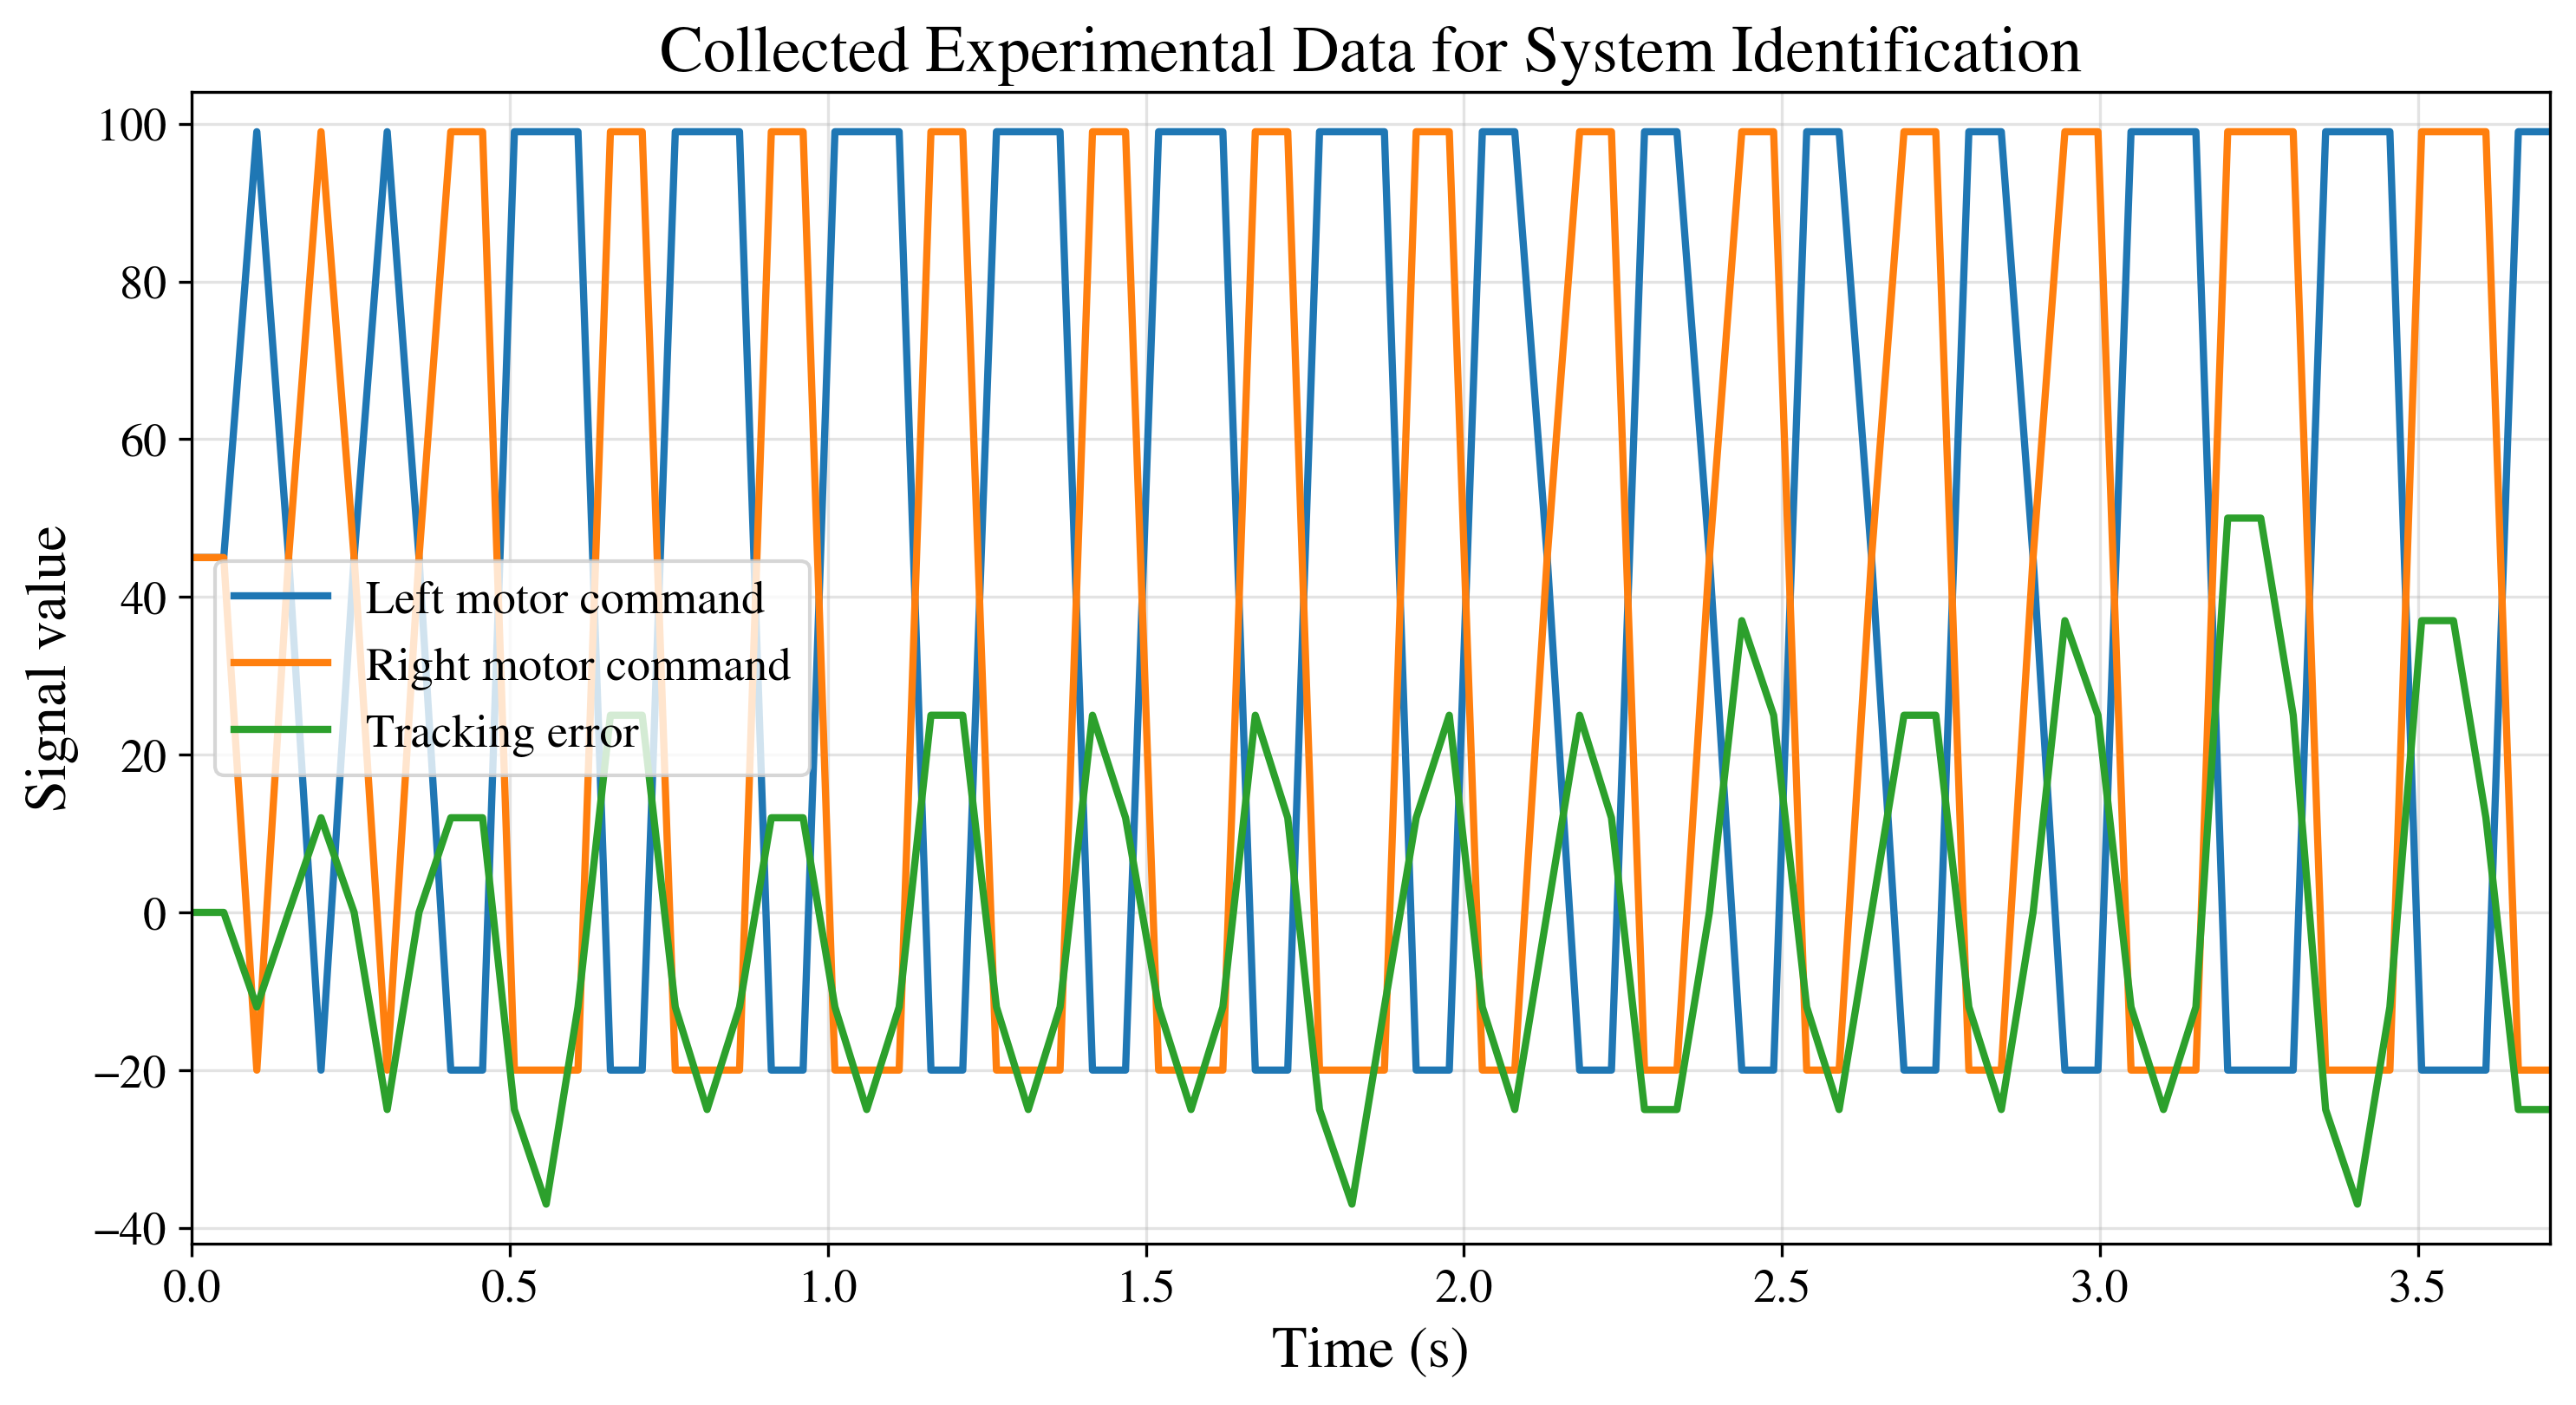
\includegraphics[width=0.9\textwidth]{Figures/system_identification_data_plot.png}
    \caption{Collected experimental data used for system identification, showing
    the left motor command, right motor command, and measured tracking error
    versus time.}
    \label{fig:sysid_data_plot_results}
\end{figure}

Using the corrected input-output definition, the final plant selected for
controller design was a second-order discrete-time transfer function given by
\[
G(z)=\frac{0.046412z^{-1}+0.204064z^{-2}}{1-0.794225z^{-1}+0.466904z^{-2}},
\]
with sampling time
\[
T_s=0.05~\text{s}.
\]

The prediction capability of the identified model was then checked by applying
the recorded steering input sequence to the transfer function and comparing the
predicted output with the measured tracking error. As shown in
Figure~\ref{fig:tf_prediction}, the model follows the main trend of the measured
response, although some mismatch remains. The resulting fit was approximately
\(56.1\%\), with an RMSE of about \(9.77\). This indicates that the identified
model captured the dominant robot dynamics well enough for controller design,
even though it did not represent all practical nonlinear effects.

\begin{figure}[htbp]
    \centering
    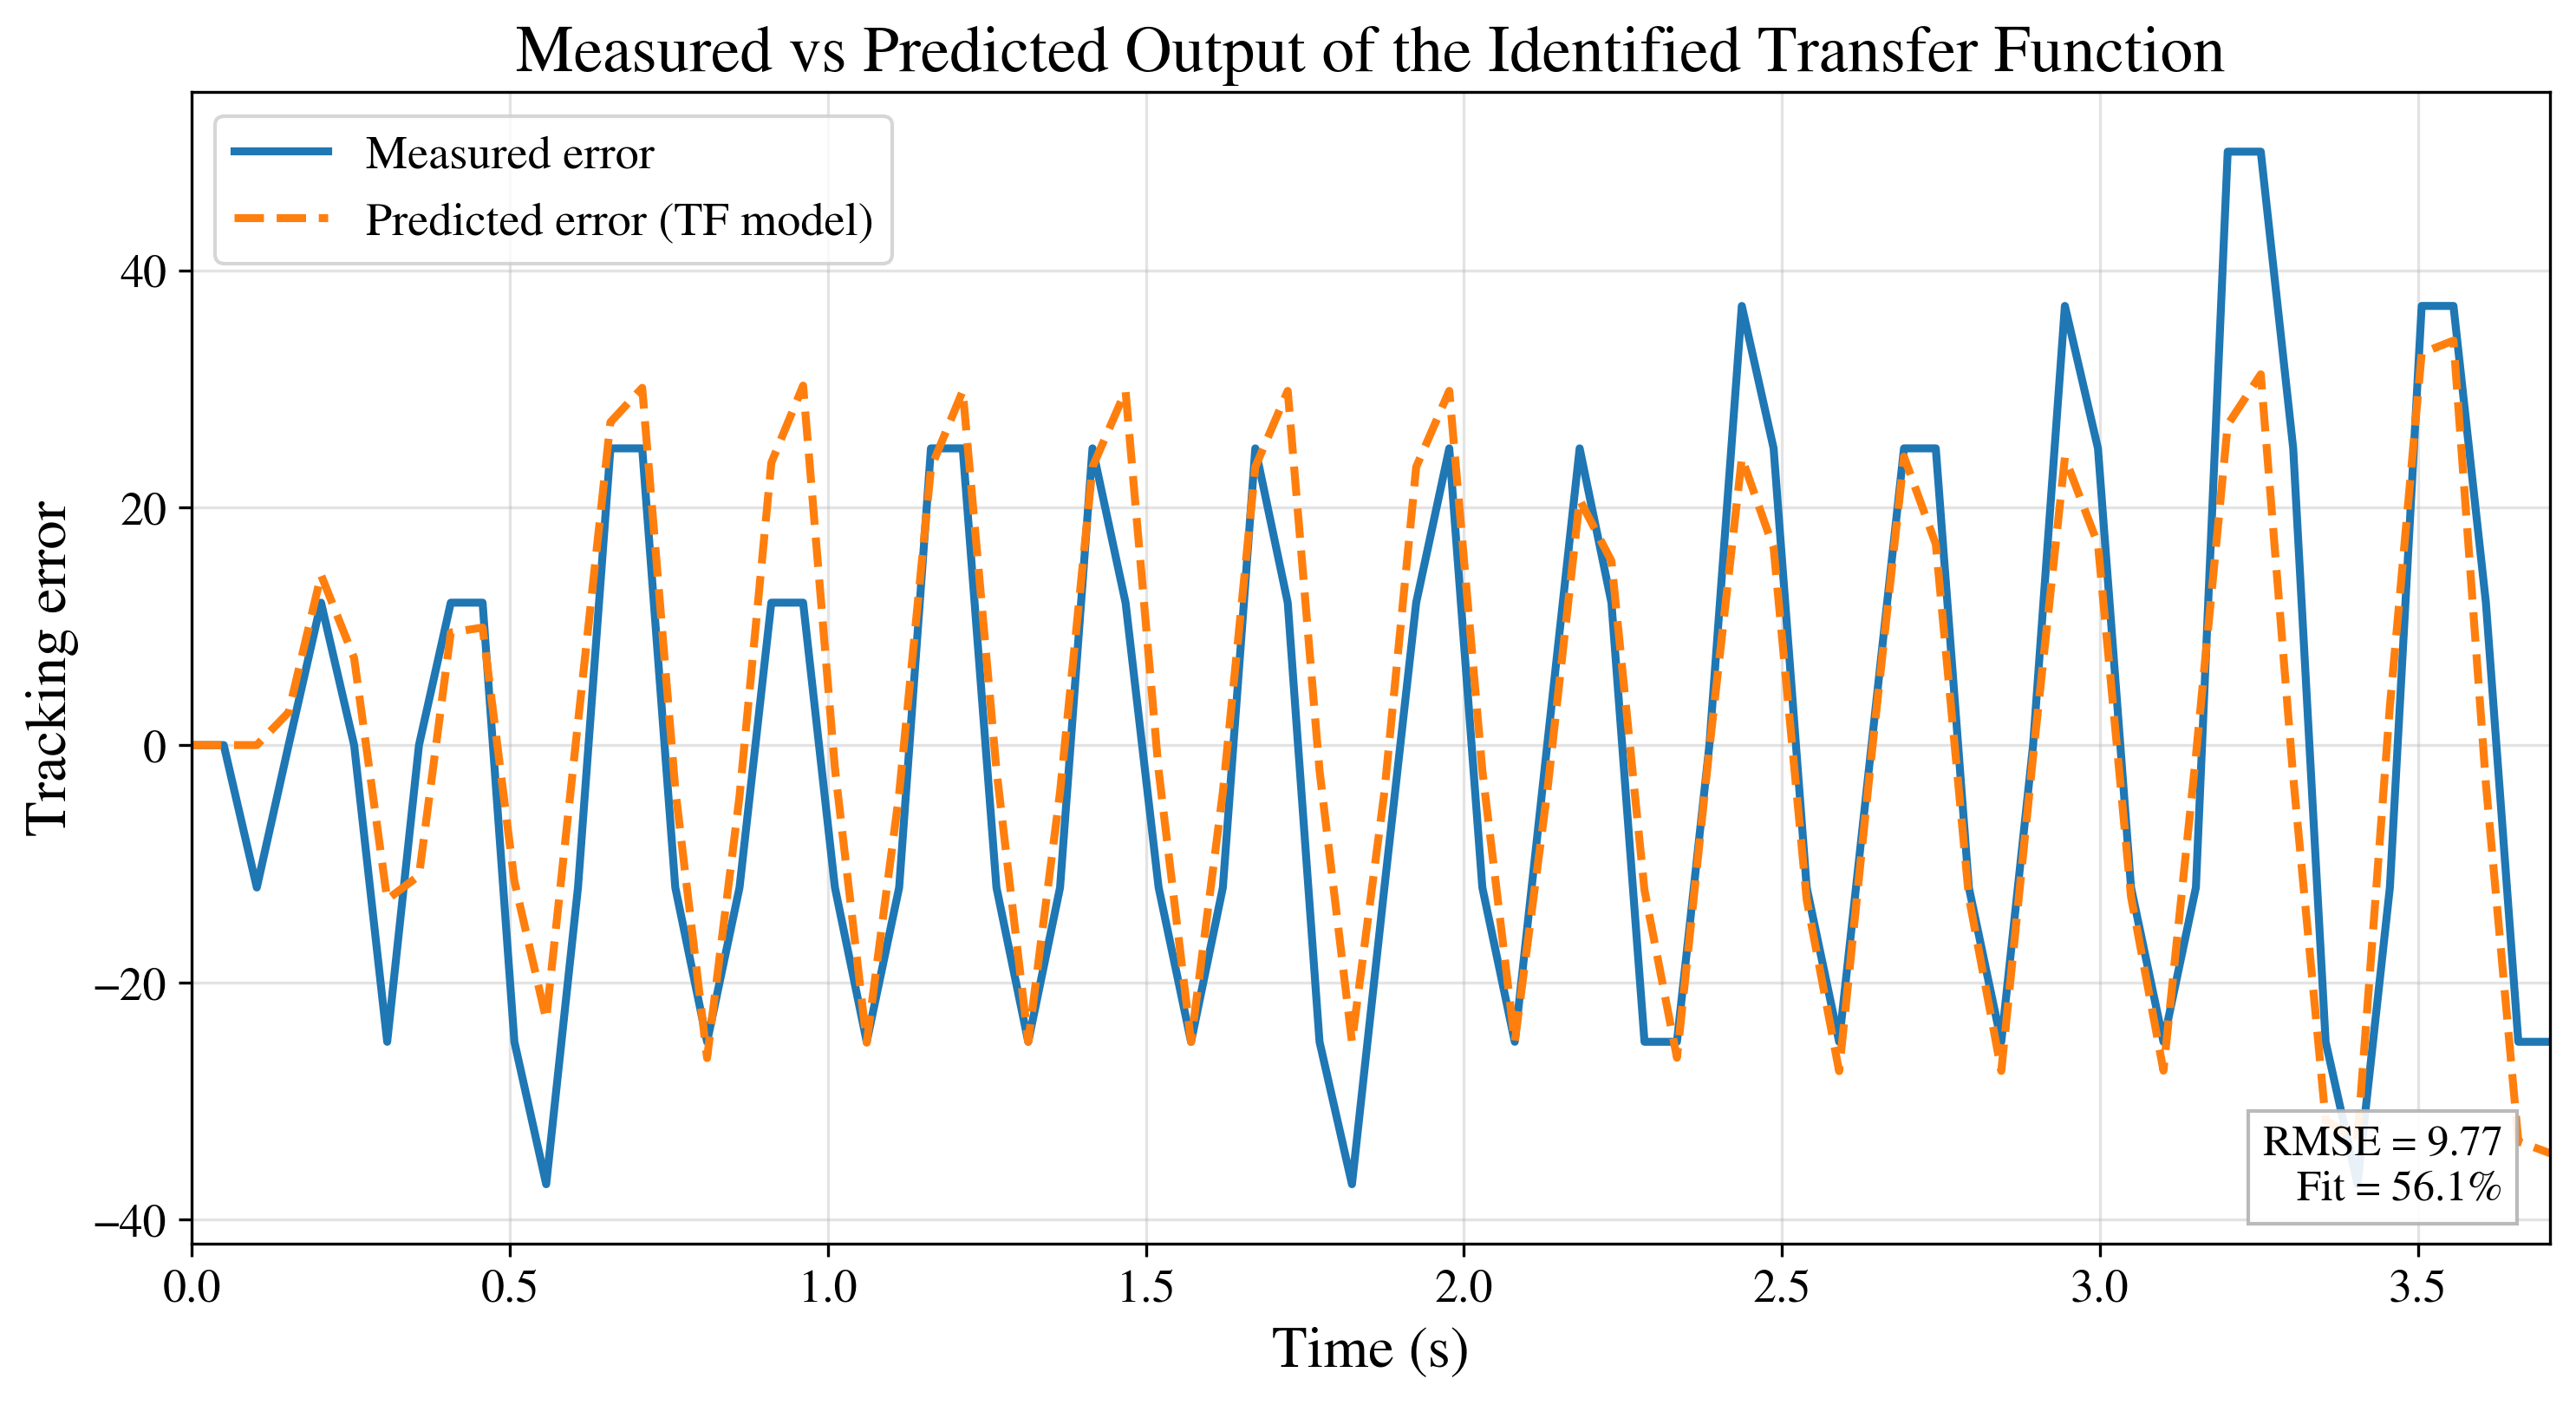
\includegraphics[width=0.9\textwidth]{Figures/tf_prediction_vs_actual_plot.png}
    \caption{Comparison between measured tracking error and the output predicted
    by the identified transfer-function model for the same input sequence.}
    \label{fig:tf_prediction}
\end{figure}

Based on this model, MATLAB PID Tuner provided the final controller parameters
\[
K_P=1.1639,\qquad K_I=1.48,\qquad K_D=-1.2571,
\]
with derivative filter coefficient
\[
N=0.64316.
\]
In simulation, the tuned closed-loop response was stable and non-oscillatory,
with zero overshoot, a rise time of about \(3.8\)~s, and a settling time of
about \(8.8\)~s.

The tuned gains were then implemented on the physical robot and tested on the
line-following track. Figure~\ref{fig:pid_validation_dual_axis} shows the
experimental validation data obtained during this run. The steering input and
measured tracking error are plotted together against time. The robot remained on
the track and the error stayed bounded throughout the experiment, confirming
that the identified model was sufficient to obtain a working controller.
However, the hardware response was less accurate than the simulated one. From
the recorded data, the measured error ranged from \(-75\) to \(+75\), with a
mean absolute error of approximately \(34\) and an RMSE of approximately
\(40.9\). The average sampling interval during the run was about
\(50.7\)~ms, which is consistent with the intended discrete-time
implementation.

\begin{figure}[htbp]
    \centering
    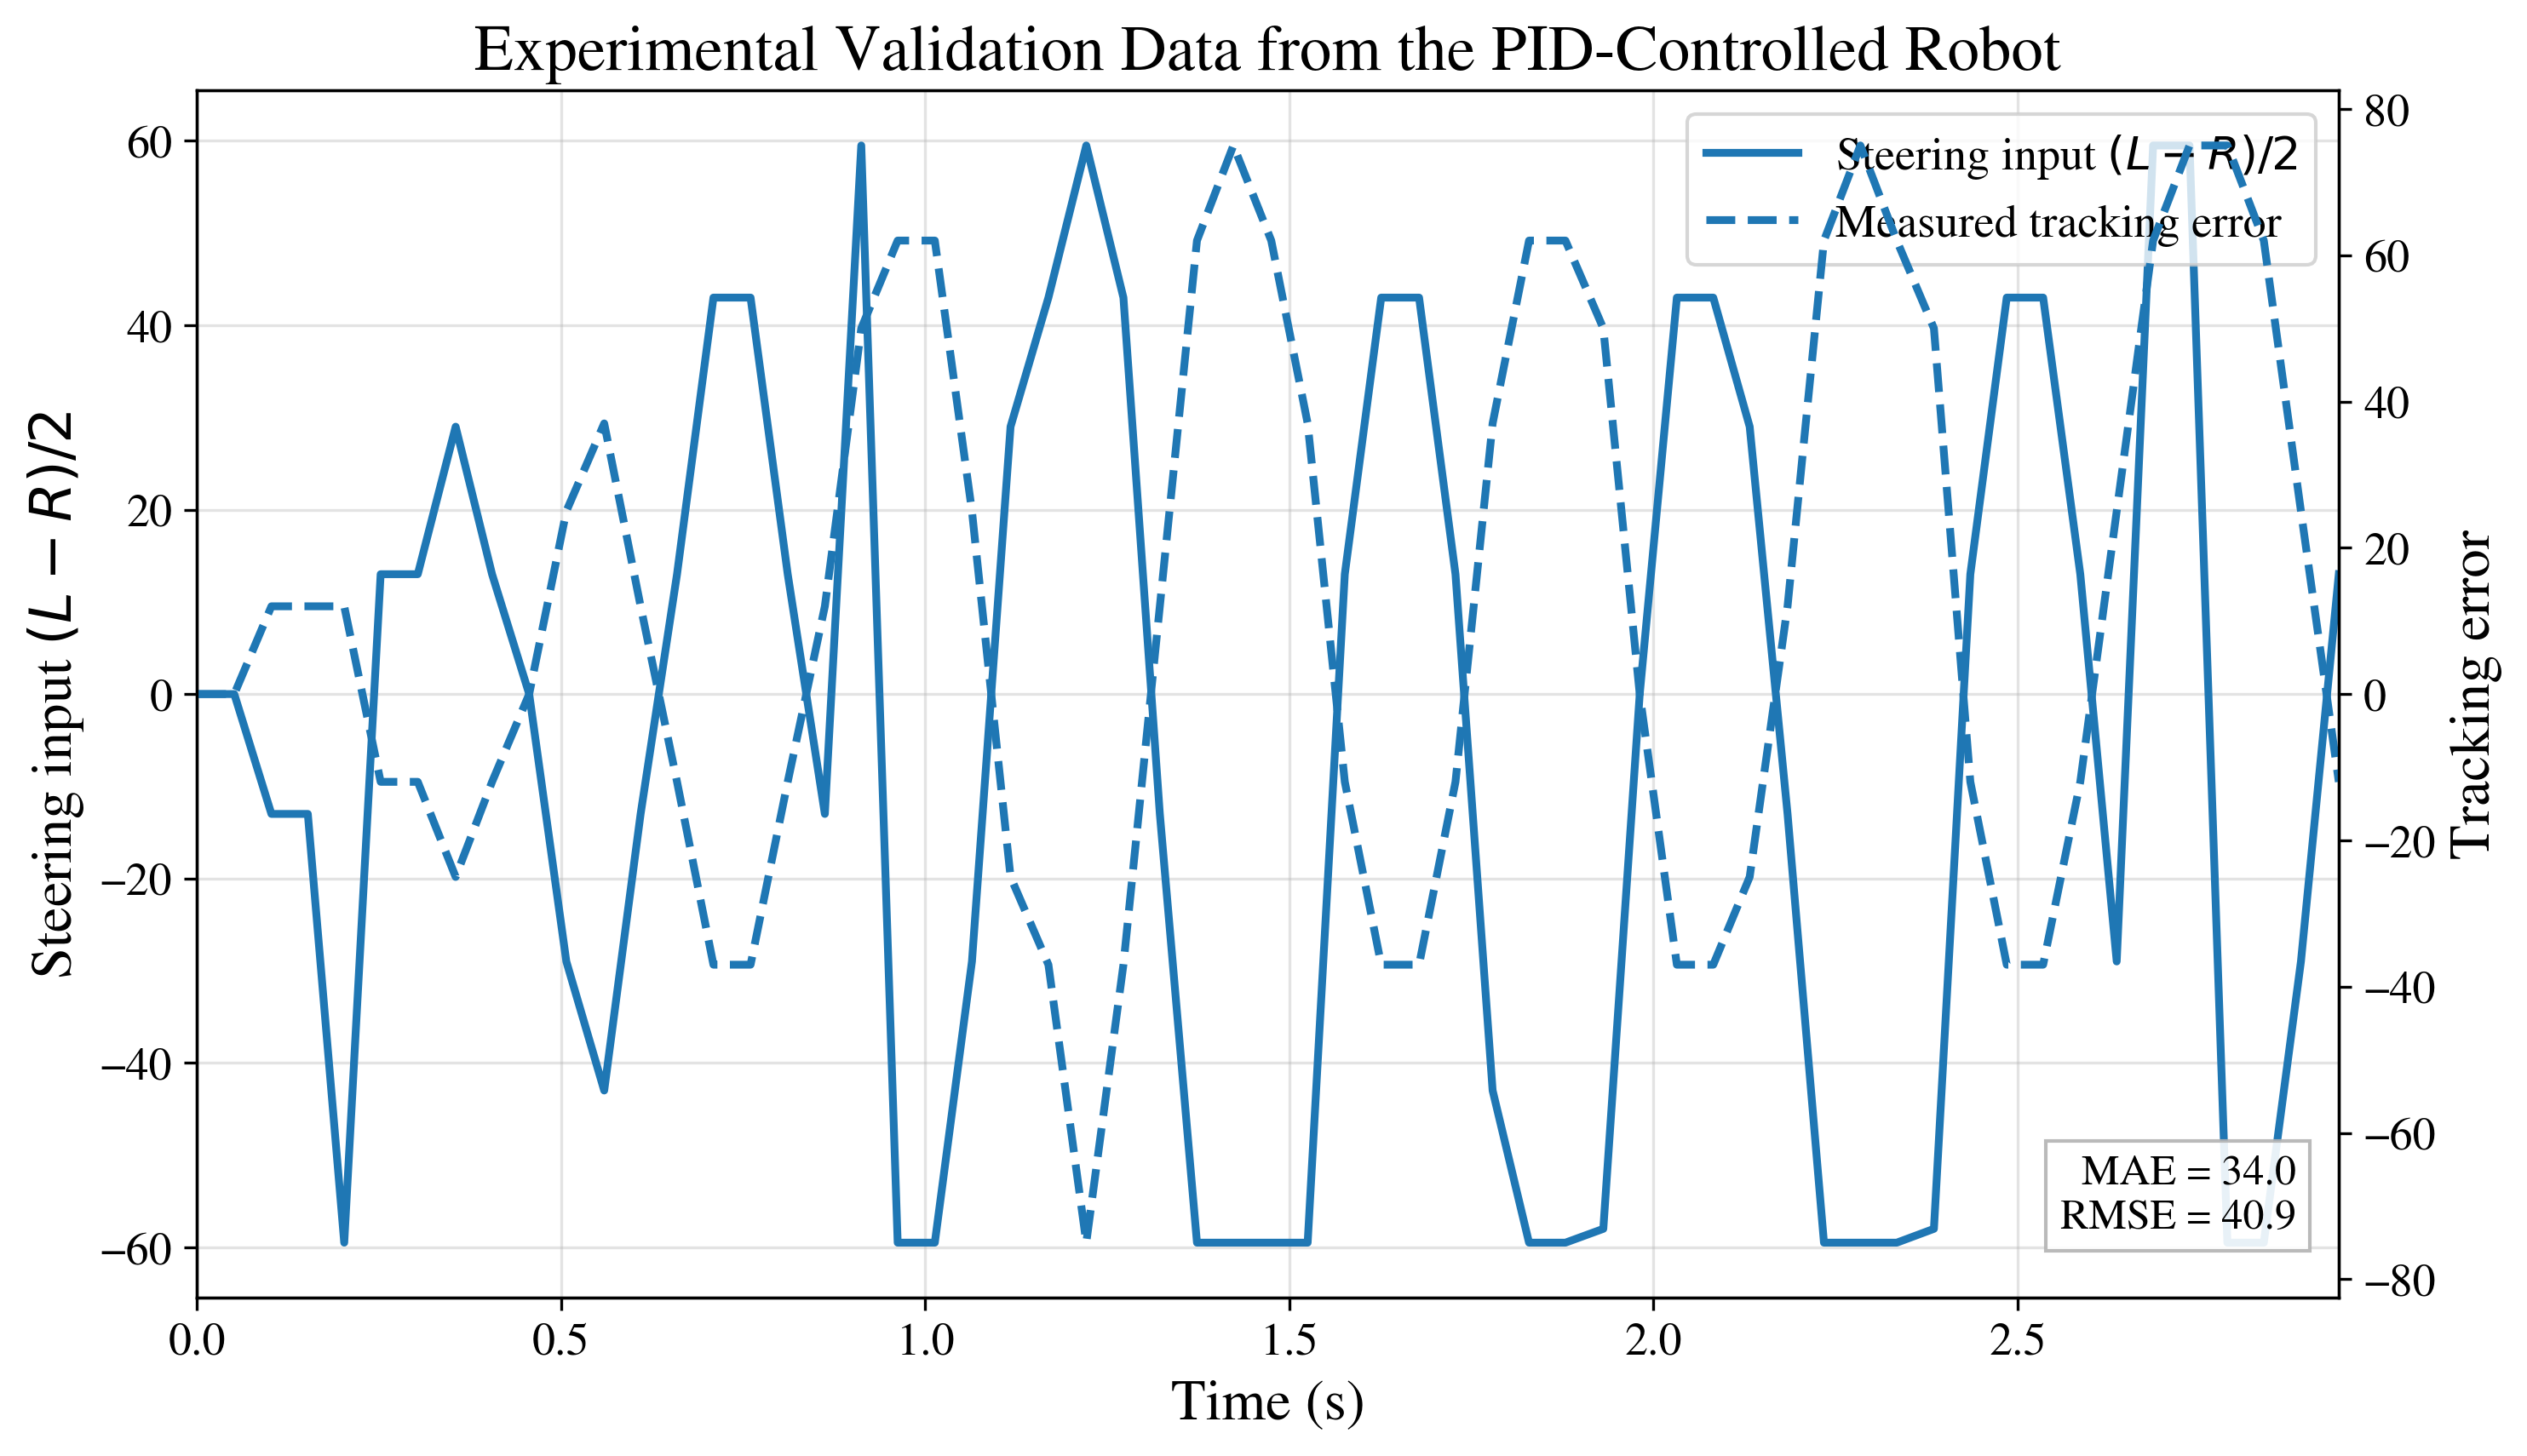
\includegraphics[width=0.9\textwidth]{Figures/pid_validation_input_error_dual_axis.png}
    \caption{Experimental validation data obtained from the robot using the PID
    gains tuned from the identified transfer-function model. The steering input
    \((L-R)/2\) and the measured tracking error are plotted against time.}
    \label{fig:pid_validation_dual_axis}
\end{figure}

\newpage
\chapter{DISCUSSIONS}

The results show that the second-order transfer-function model captured the main behaviour of the robot well enough for simulation-based PID design. This suggests that a simple linear model can still serve as a useful control-oriented approximation for a low-cost line-following robot.

The PID controller tuned in MATLAB gave a good response in simulation, but the hardware test showed lower tracking accuracy. Although the robot remained on the line, the measured error was still large in several parts of the run. The recorded data also show repeated operation near unequal wheel-speed limits during stronger corrections. This indicates that the real robot is influenced by motor dead-zone, actuator saturation, sensor quantisation, and other nonlinear effects that were not fully captured by the identified linear model.

Overall, the main contribution of this work is not perfect tracking, but the demonstration that real experimental data can be used to obtain a practical plant model and a working PID controller in a more systematic way than manual tuning alone. At the same time, the difference between simulation and hardware response highlights the limitations of the selected linear model for representing the full behaviour of the real robot.
\newpage
\chapter{CONCLUSIONS, LIMITATIONS, AND FUTURE RESEARCH DIRECTIONS}

This project developed a systematic workflow for the modeling and control of a differential-drive line-following robot. A 14-element infrared sensor array was used to estimate line position, and experimental telemetry from the robot was used to identify a discrete-time plant model. The identified model was then used for PID tuning in MATLAB, and the tuned controller was implemented on the physical robot.

The study showed that an identification-based approach can be used to obtain a practical controller for a low-cost line-following robot without relying only on manual tuning.

The main limitation of the work is that the final model is linear, while the real robot exhibits nonlinear effects such as motor dead-zone, actuator saturation, sensor quantisation, and changing track conditions. Because of these effects, the experimental response did not fully match the simulated response.

Future work may focus on improving the plant model and controller design. Possible directions include nonlinear system identification, gain scheduling for different operating speeds, explicit treatment of actuator saturation, and comparison of PID control with other control strategies.
\backmatter
\renewcommand\bibname{REFERENCES}
\newpage
\phantomsection \label{refs}
\addcontentsline{toc}{part}{REFERENCES}
\printbibliography[title={REFERENCES}]

% \appendix
% \newpage
% \begin{center}
% \HeadingR{\MakeUppercase{Appendices}}
% \end{center}
% \addcontentsline{toc}{part}{\MakeUppercase{APPENDICES}}

% \section*{Data availability}
% Write about the availability of the datasets used in this project.

% \section*{Code availability}
% Indicate and link the public repository of the codes used in this project.

\end{document}
